\documentclass[10pt]{article}
\usepackage{amsmath,graphicx,hyperref,tcolorbox,geometry}
\geometry{a4paper,left=2.54cm,right=2.54cm,top=2.1cm,bottom=2.1cm}
\hypersetup{colorlinks=true,linkcolor=blue,urlcolor=blue}
\setlength{\parindent}{2em}
\setlength{\parskip}{0pt}
\newtcolorbox{keybox}[1][]{colback=blue!3!white,colframe=blue!40!black,fonttitle=\bfseries,title={#1}}
\title{\textbf{Suppressed Density Fluctuations in a Disk-Sensing Brownian Model}}
\author{Notes on the model of Wu et al.}
\date{}
\begin{document}
\maketitle
\vspace{-2em}
\section{The particle model and a stable suppression regime}
Wu et al.\ [1] consider Brownian displacements whose local variance is controlled by the number of particles in a sensing disk. In the paper's dimensionless units, the perceived density and diffusivity are
\begin{equation}
 P_i=\frac{n_i}{\pi R^2},\qquad D(P_i)=\chi+(P_i-1)^2,
 \qquad \chi=0.002,
 \label{eq:model}
\end{equation}
where the disk count $n_i$ includes particle $i$ itself. Our particle simulations use the same It\^{o} Euler--Maruyama update, $R=5$, $\Delta t=0.05$, and periodic squares of side $L=40$ or $80$. Following Ref.\ [1], the mean density $\rho_0=N/L^2$ takes the values $1.6,2,3$.

For a homogeneous reference state, replace the particle count by the normalized disk convolution $P=W_R*\rho$, where $W_R(r)=\Theta(R-r)/(\pi R^2)$. Linearizing the It\^{o}--Dean density equation about $\rho=\rho_0$ gives
\begin{equation}
 \bar D=\chi+(\rho_0-1)^2,\quad g=D'(\rho_0)=2(\rho_0-1),\quad
 \widehat W_R(k)=\frac{2J_1(kR)}{kR},\quad
 S_{\rm lin}(k)=\frac{\bar D}{\bar D+\rho_0g\widehat W_R(k)}.
 \label{eq:linear}
\end{equation}
Here $\bar D=D(\rho_0)$ is the diffusivity at the mean density, and $g$ is its local sensitivity to perceived density. The factor $\widehat W_R(k)$ is the Fourier transform of the normalized sensing disk at wave number $k$; $J_1$ is the first-order Bessel function. Finally, $S_{\rm lin}(k)$ is the predicted structure factor, normalized so an uncorrelated state has $S=1$. It follows from the stationary covariance of each conserved Gaussian Fourier mode and requires $\bar D+\rho_0g\widehat W_R(k)>0$ for all allowed modes. This is a reference for a stable homogeneous state, not an exact spectrum of the nonlinear particle process. The continuum replacement also neglects the tagged-particle self-count shift $1/(\pi R^2)$.

For $\rho_0>1$, $g>0$ and $S_{\rm lin}(0^+)=1/(1+B)<1$, where $B=\rho_0g/\bar D$. The negative minimum of the disk transform is approximately $-0.13228$, so the continuum homogeneous state remains linearly stable throughout the resolved band if $B<7.56$. Here $B\simeq5.30,3.99,3.00$ for $\rho_0=1.6,2,3$, respectively. These are the conditions under which suppression relative to the uncorrelated baseline $S=1$ can be assessed without first crossing a linear instability.

\begin{figure}[h!]
 \centering
 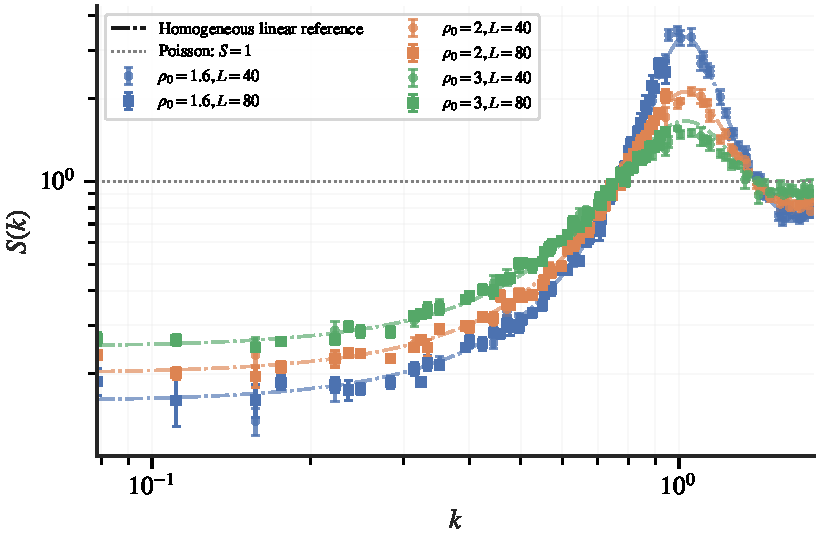
\includegraphics[width=.60\linewidth]{density_scan_loglog_scaling.pdf}
 \vspace{-1em}
 \caption{Measured structure factor versus $k$ (points). Dot--dash curves are the homogeneous linear reference, Eq.~\eqref{eq:linear}; circles and squares denote $L=40$ and $80$. The dotted line marks the uncorrelated baseline $S=1$.}
 \label{fig:sk}
\end{figure}

\clearpage
\section{Numerical evidence and its limits}
Figure~\ref{fig:sk} shows a marked drop below $S=1$ as $k$ decreases through the sensing-scale crossover. Fits to the saved $L=80$ spectra over the finite interval $0.5\leq k\leq1$ give effective log--log slopes of about $3.61,2.76,1.89$ for $\rho_0=1.6,2,3$; they are not asymptotic exponents. At the smaller modes supplied by $L=80$, $k_{\min}R=2\pi R/L\simeq0.393$ and the measured first-shell values are
\begin{equation}
 S(k_{\min})=0.187\pm0.021\quad(\rho_0=1.6),\qquad
 0.235\pm0.045\quad(\rho_0=2),\qquad
 0.268\pm0.014\quad(\rho_0=3).
 \label{eq:data}
\end{equation}
Errors are standard errors from six time blocks over $500<t\leq1500$ in one trajectory per parameter set; they are not independent-seed uncertainties. The $L=40$ spectra extend to larger $k$ and agree broadly with $L=80$ in their overlap.

\begin{figure}[h!]
 \centering
 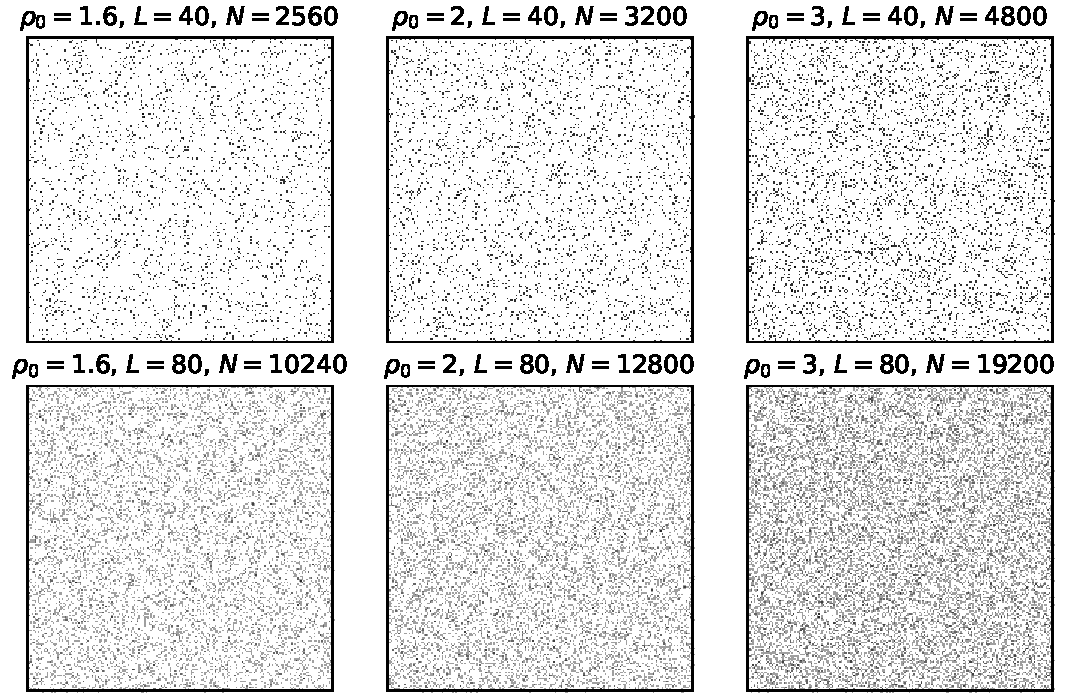
\includegraphics[width=.82\linewidth]{six_final_snapshots.pdf}
 \vspace{-1em}
 \caption{Final particle positions at $t=1500$ for the six runs in Fig.~\ref{fig:sk}: columns $\rho_0=1.6,2,3$; rows $L=40,80$. Each panel displays the whole periodic square. The suppression claim comes from $S(k)$, not visual appearance.}
 \label{fig:snap}
\end{figure}

\begin{keybox}[Conclusion]
The equal-weight disk-sensing model of Ref.\ [1] \emph{can suppress density fluctuations} over measured long wavelengths when $\rho_0>1$, the positive response $g$ is strong enough to reduce $S$, and the homogeneous state remains stable. This does not require inverse-distance sensing. Finite $R$ and finite $B$ give a positive $k\to0$ plateau in the linear theory; the finite-interval slopes in Fig.~\ref{fig:sk} therefore do not establish asymptotic hyperuniformity.
\end{keybox}

\smallskip
{\small [1] B. Wu et al., \emph{Nonlocal Sensing Drives Hybrid Phase Separation in Brownian Matter}, \href{https://arxiv.org/abs/2606.21464}{arXiv:2606.21464v1} (2026), especially the particle protocol in Supplemental Material S1.}
\end{document}
